\chapter{The Three-body Problem}
Two-body scattering processes basically concern two different situations, elastic and inelastic collisions. For the three-body problem, solving the three-body Schr{\"o}dinger equation is more involved. The enhanced complexity is mainly due to the increased number of fragmentation channels in the scattering processes. In addition to the triatomic fragmentation channel (1+1+1), there are three possible atom-dimer fragmenation channels (1+2). This makes the construction of permutation symmetric wavefunctions highly non-trivial. 

There are different routes for solving the three-body problem and they involve either solving the three-body Schr{\"o}dinger equation or solving the Faddeev equation, which is equivalent to solving the three-body Schr{\"o}dinger equation in configuration space. Irrespective of the specific method of choice for solving the three-body system, most approaches start with the same steps. These include separating out the center-of-mass motion and then defining a set of relative coordinates. A convenient choice for the three-body problem is mass normalized Jacobi coordinates, since this removes the mass factors in the kinetic energy operator. Introducing hyperspherical coordinates in combination with an adiabatic representation are then used to reduce the problem of three colliding atoms to dynamics on a set of coupled adiabatic hyperspherical potentials.

Atomic units\footnote{There are four fundamental atomic units -- the electron rest mass $m_e$, the elementary charge $e$, the reduced Planck's constant $\hbar$, and the Coulomb force constant $k_e$ -- whose numerical values are unity by definition, i.e. $m_e = e = \hbar = k_e = 1$. Derived atomic units include dimensions of length and energy, which are expressed in terms of the Bohr radius $a_0$ and the Hartree $E_h$.    } (a.u.) will be used in the following chapters. 

\section{Mass Normalized Jacobi Coordinates}\label{MNJC}
The spatial position of three particles in $\mathbb{R}^3$ are fixed by nine coordinates $x_{\alpha}^{i}$, where $i(=1,2,3)$ labels the particles, and $\alpha(=1,2,3)$ their Cartesian space coordinates. Let $\mathbf{x}_i$ and $m_{i}$ be the position vector and mass of the $i$th particle in the laboratory frame. If the total mass $M$, the three particle reduced mass $\mu$, and the normalizing constants $d_{k}$ $(k=1,2,3)$ are defined by

\begin{align}
M &= \sum_{i=1}^{3}m_i,  \label{eq:3,1} \\
\mu^2 &= \prod_{i=1}^{3}m_i/M,  \label{eq:3,2}\\
d_k^2 &= \frac{m_k}{\mu}\frac{(m_i+m_j)}{M},  \label{eq:3,3}
\end{align}
then a set of mass scaled Jacobi coordinates and the center-of-mass coordinate can be defined as

\begin{align}
\mathbf{r}_k &= d^{-1}_k(\mathbf{x}_{j}-\mathbf{x}_{i}),  \label{eq:4_1} \\
\mathbf{R}_k &= d_k\Big[\mathbf{x}_{k}-\frac{(m_{i}\mathbf{x}_{i}+m_{j}\mathbf{x}_{j})}{m_{i}+m_{j}}\Big],  \label{eq:4_2}\\
\mathbf{X}_{cm} &= \frac{1}{M} \sum_{i=1}^{3} m_{i} \mathbf{x}_{i},  \label{eq:4_3}
\end{align}   
in which the indices $i,j,k$ are cyclic permutations of $(1,2,3)$ and where $\mathbf{r}_k$ is the scaled vector from particle $i$ to $j$, and $\mathbf{R}_k$ is the scaled vector from the centre-of-mass of the pair $ij$ to particle $k$, see \cref{fig:1}.
\begin{figure}
	\centering
	 \documentclass{standalone}
 \usepackage{tikz}
 \usepackage{tikz-3dplot}
 \usetikzlibrary{calc}
 
 \begin{document}
 
  %Angle Definitions
%-----------------

%set the plot display orientation
%synatax: \tdplotsetdisplay{\theta_d}{\phi_d}
\tdplotsetmaincoords{60}{110}

%define polar coordinates for some vector
%TODO: look into using 3d spherical coordinate system
\pgfmathsetmacro{\rvec}{.8}
\pgfmathsetmacro{\thetavec}{30}
\pgfmathsetmacro{\phivec}{80}

\pgfmathsetmacro{\rveca}{.8}
\pgfmathsetmacro{\thetaveca}{50}
\pgfmathsetmacro{\phiveca}{320}

\pgfmathsetmacro{\rvecb}{.8}
\pgfmathsetmacro{\thetavecb}{50}
\pgfmathsetmacro{\phivecb}{40}


%start tikz picture, and use the tdplot_main_coords style to implement the display 
%coordinate transformation provided by 3dplot
\begin{tikzpicture}[scale=5,tdplot_main_coords]

%set up some coordinates 
%-----------------------
\coordinate (O) at (0,0,0);

%determine a coordinate (P) using (r,\theta,\phi) coordinates.  This command
%also determines (Pxy), (Pxz), and (Pyz): the xy-, xz-, and yz-projections
%of the point (P).
%syntax: \tdplotsetcoord{Coordinate name without parentheses}{r}{\theta}{\phi}
\tdplotsetcoord{P}{\rvec}{\thetavec}{\phivec}
\tdplotsetcoord{F}{\rveca}{\thetaveca}{\phiveca}
\tdplotsetcoord{R}{\rvecb}{\thetavecb}{\phivecb}
\coordinate (M) at ($ (P) !.5! (R) $);


%draw figure contents
%--------------------

%draw the main coordinate system axes
\draw[thick,->] (0,0,0) -- (1,0,0) node[anchor=north east]{$x$};
\draw[thick,->] (0,0,0) -- (0,1,0) node[anchor=north west]{$y$};
\draw[thick,->] (0,0,0) -- (0,0,1) node[anchor=south]{$z$};
%draw a vector from origin to point (P) 
\draw[-stealth,color=red] (O) -- (P) node[pos=0.5, right]{$x_{i}$};
\draw[-stealth,color=red] (O) -- (F) node[pos=0.5, right]{$x_{k}$};
\draw[-stealth,color=red] (O) -- (R) node[pos=0.5, right]{$x_{j}$};

\draw[thick,->,color=blue] (P) -- (R) node[pos=0.5, right]{$x_{ij}$};
\draw[thick,->,color=blue] (M) -- (F) node[pos=0.5, below]{$x_{ij,k}$};
%\draw[-stealth,color=red] (O) -- (R);

%draw projection on xy plane, and a connecting line
\draw[dashed, color=red] (O) -- (Pxy);
\draw[dashed, color=red] (P) -- (Pxy);

\draw[dashed, color=red] (O) -- (Fxy);
\draw[dashed, color=red] (F) -- (Fxy);

\draw[dashed, color=red] (O) -- (Rxy);
\draw[dashed, color=red] (R) -- (Rxy);

%draw the angle \phi, and label it
%syntax: \tdplotdrawarc[coordinate frame, draw options]{center point}{r}{angle}{label options}{label}
\tdplotdrawarc{(O)}{0.8}{0}{\phivec}{anchor=north}{$\phi_i$}
\tdplotdrawarc{(O)}{0.2}{0}{\phiveca}{anchor=north}{$\phi_j$}
\tdplotdrawarc{(O)}{0.4}{0}{\phivecb}{anchor=north}{$\phi_k$}


%set the rotated coordinate system so the x'-y' plane lies within the
%"theta plane" of the main coordinate system
%syntax: \tdplotsetthetaplanecoords{\phi}
\tdplotsetthetaplanecoords{\phivec}

%draw theta arc and label, using rotated coordinate system
\tdplotdrawarc[tdplot_rotated_coords]{(0,0,0)}{0.8}{0}{\thetavec}{anchor=south west}{$\theta_i$}

%draw some dashed arcs, demonstrating direct arc drawing
\draw[dashed,tdplot_rotated_coords] (\rvec,0,0) arc (0:90:\rvec);
\draw[dashed] (\rvec,0,0) arc (0:90:\rvec);


\tdplotsetthetaplanecoords{\phiveca}
\tdplotdrawarc[tdplot_rotated_coords]{(0,0,0)}{0.8}{0}{\thetaveca}{anchor=south east}{$\theta_k$}


%draw some dashed arcs, demonstrating direct arc drawing
\draw[dashed,tdplot_rotated_coords] (\rveca,0,0) arc (0:90:\rveca);
\draw[dashed] (\rveca,0,0) arc (0:\phiveca:\rveca);

\tdplotsetthetaplanecoords{\phivecb}
\tdplotdrawarc[tdplot_rotated_coords]{(0,0,0)}{0.8}{0}{\thetavecb}{anchor=south east}{$\theta_j$}


%draw some dashed arcs, demonstrating direct arc drawing
\draw[dashed,tdplot_rotated_coords] (\rvecb,0,0) arc (0:90:\rvecb);
\draw[dashed] (\rvecb,0,0) arc (0:90:\rvecb);


\end{tikzpicture}
\end{document}
	\caption{Spatial positions of three particles.}
	\label{fig:1}
\end{figure}
The kinetic energy operator for the three particles in the laboratory frame, as given by 

\begin{equation}\label{eq:5}
T = -\frac{1}{2} \sum_{i=1}^{3} m_{i}^{-1} \nabla^{2}_{\mathbf{x}_{i}}, 
\end{equation}
will subsequently transform into

\begin{equation}\label{eq:6}
T = -\frac{1}{2\mu} \Big(\nabla^{2}_{\mathbf{r}_{k}}+\nabla^{2}_{\mathbf{R}_{k}}\Big) - \frac{1}{2 M}\nabla^{2}_{\mathbf{X}_{cm}}. 
\end{equation}
Now, since the interaction $V(\mathbf{r}_k,\mathbf{R}_k)$ does not depend on $\mathbf{X}_{cm}$, the center-of-mass motion decouples from the internal motion in the Schr{\"o}dinger equation if we write the wavefunction as

\begin{equation}
\Psi(\mathbf{r}_k,\mathbf{R}_k,\mathbf{X}_{cm}) = \varphi(\mathbf{X}_{cm})\psi(\mathbf{r}_k,\mathbf{R}_k),
\end{equation}
so that

\begin{equation}
(H_{cm} + H_{int})\varphi_{k}(\mathbf{X}_{cm})\psi_{n}(\mathbf{r}_k,\mathbf{R}_k) = (E_k^{cm} + E_n^{int})\varphi_{k}(\mathbf{X}_{cm})\psi_{n}(\mathbf{r}_k,\mathbf{R}_k).
\end{equation}
Henceforth, we will only consider the internal motion part of the  Schr{\"o}dinger equation. To clarify the notations, from now on wavefunctions and energies labelled $\Psi$ and $E$ refers to the internal eigenstates and eigenenergies, which were labelled $\psi$ and $E^{int}$ previously. 

\begin{figure}
	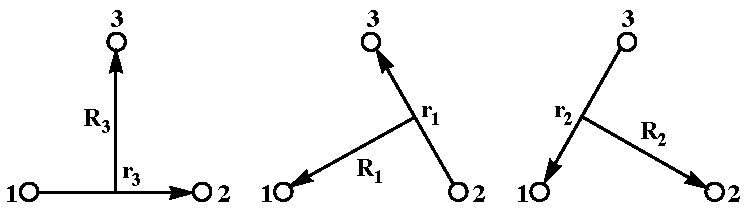
\includegraphics[width=\linewidth]{jacobii.pdf}
	\caption{Illustration of the three different Jacobi coordinate sets.}
	\label{fig:2}
\end{figure}

There are three possible ways to construct the Jacobi coordinates described above, see \cref{fig:2}. Each set transforms into one of the other sets the by exchange of particles. To be able to describe permutations in a system with mass-scaled coordinates it is useful to introduce angles defined by the particle masses \cite{Smith1962}. If an even permutation $(ijk)$ of the set $(123)$ is considered, then the obtuse angle $\beta_{ij}$ has the properties

\begin{subequations}
	\begin{align}
	&\beta_{ij} = -\beta_{ji}, \quad \beta_{ii} = 0,\\
	&\tan\beta_{ij} = -m_k/\mu,\\
	&d_{i}d_{j} \sin\beta_{ij} = 1,\\
	&d_{i}d_{j} m_{k} \cos\beta_{ij} = -\mu,\\
	&\beta_{12}+\beta_{23}+\beta_{31} = 2\pi.
	\end{align}
\end{subequations}
Orthogonal transformations within the coordinate set are then given by 

\begin{equation}
\begin{pmatrix}
\mathbf{r}_j\\
\mathbf{R}_j
\end{pmatrix}
=
\begin{pmatrix}
\cos\beta_{ij} & \sin\beta_{ij}\\
-\sin\beta_{ij} & \cos\beta_{ij}
\end{pmatrix}
\begin{pmatrix}
\mathbf{r}_i\\
\mathbf{R}_i
\end{pmatrix}.
\end{equation}

\section{The Hyperspherical Method}
The next common step in the theoretical framework to describe systems of three particles is to introduce hyperspherical coordinates. The components of the two vectors $\mathbf{r}$ and $\mathbf{R}$ are combined into a single, six-dimensional position vector $\mathbf{q}$. The components of this vector can be regarded as the cartesian components of a point in $\mathbb{R}^{6}$. The motion of a three particle system is thus equivalent to the motion of a single particle, with the reduced mass $\mu$, in six-dimensional Euclidean space. The polar coordinates of this point particle are given by one hyperradial coordinate $\rho$, and five hyperangular coordinates, collectively labelled $\Omega$. Three of these angles $\alpha, \beta, \gamma$ are usually chosen as the Euler angles that specify the  orientation of the body-fixed axis system -- i.e. the triangle formed by the three particles -- relative to a space-fixed coordinate frame. These are the external coordinates of the system. The internal coordinates are the hyperradius, which describes the overall size of the system, and the remaining two hyperangles, which describe the shape of the triangle formed by the  three particles. 

Hyperspherical coordinates are useful for describing fragmentation problems. Fragmentation processes of the system into any one of the possible channels are described by the hyperradius becoming very large $(\rho \rightarrow \infty)$, while the hyperangles distinguish between the different fragmentation channels. The hyperradius is invariant under both rotations and particle permutations, and for the three-body problem it is defined by

\begin{equation}
\rho = \Big(\mathbf{r}^{2} + \mathbf{R}^{2}\Big)^{1/2}, \quad 0\leq \rho < \infty.
\end{equation} 

In contrast to the hyperradius there is no unique way to define the hyperangles and the various definitions are not in general invariant under particle permutations. The most common choises of parametrizing the hypersphere fall into two distinct categories: Delves coordinates, and (democratic) Smith-Whitten coordinates. A brief overview of these coordinates is given in \cref{delvescoord,smith_whitten} and a more thorough description can be found in \cref{delves,smith}.

Independent of the specific choise of hyperangular coordinates, after scaling the total wave function by a factor $\rho^{5/2}$ the three-body Schr{\"o}dinger equation in terms of general hyperspherical coordinates is written

\begin{equation}\label{eq:schrodinger_general}
\bigg(-\frac{1}{2 \mu}\frac{\partial^2}{\partial \rho^2} + \frac{ \Lambda^2 + \frac{15}{4}}{2 \mu \rho^{2}}+ V(\rho,\Omega)\bigg)\psi(\rho,\Omega) = E\psi(\rho,\Omega),
\end{equation}
where $\Lambda$ is the grand angular momentum operator.

\section{The Adiabatic Hyperspherical Representation}\label{sec:AHM}
The first step in solving \eqref{eq:schrodinger_general} is to introduce the adiabatic representation. This means expanding the solution $\psi_{n}(\rho,\Omega)$ into a complete set of orthonormal channel functions $\Phi_{\nu}(\rho;\Omega)$ that depend parametrically on $\rho$, with the radial wavefunctions $F_{\nu n}(\rho)$ as expansion coefficients. The hyperradius is treated as an adiabatic variable and the channel functions $\Phi_{\nu}$ are eigenfunctions to the adiabatic equation

\begin{equation}\label{adiabatic}
H_{ad}\Phi_{\nu}{(\rho;\Omega)} = U_{\nu}{(\rho)}\Phi_{\nu}(\rho;\Omega), 
\end{equation}
where the eigenvalues $U_{\nu}(\rho)$ are the resulting effective potental curves obtained by solving this eigenvalue equation at a number of different hyperradii, and $H_{ad}$ is the adiabatic Hamiltonian given by

\begin{equation}\label{eq:adiabitic_hamiltonian}
H_{ad} = \frac{\Lambda^2+\frac{15}{4}}{2 \mu \rho^2} + V(\rho,\Omega).
\end{equation}
The adiabatic hyperspherical potentials $U_{\nu}$ contain most of the three-body physics and can be regarded as the three-body equivalent to the Born-Oppenheimer potential in the two-body problem. The zero potential eigenfunctions $\Phi_{\nu}$ of equation \eqref{adiabatic} for three identical bosons are the Gegenbauer polynomials with eigenvalues

\begin{equation}\label{eq:gegenbauer}
U(\rho) = \frac{\lambda(\lambda + 4) + \frac{15}{4}}{2\mu \rho^2},
\end{equation} 
where $\lambda = 0, 4, 6, \ldots$ \cite{Blume2002}.
The total wave function

\begin{equation}\label{wave}
\psi_{n}(\rho,\Omega) = \sum_{\nu=0}^{\infty} F_{n\nu}(\rho)\Phi_{\nu}(\rho;\Omega),
\end{equation}
can thus be represented in terms of adiabatic states, which, in principle, yields an exact representation of the three-body Schr{\"o}dinger equation if all couplings are included. The power of this method is that the problem can be reduced to a system of coupled ordinary differential equations where the major effort lies in solving the adiabatic equation. Substituting \eqref{wave} into \eqref{eq:schrodinger_general} and projecting out $\Phi_{\nu'}$ by multiplying the conjugate transpose $\Phi_{\nu}^{\dagger}$ to the left and integrating over the hyperanglular coordinates results in an infinite set of coupled differential equations in $\rho$, which reads

\begin{align}\label{fullhamiltonian}
\bigg(-\frac{1}{2 \mu}\frac{\partial^2}{ \partial \rho^2} + U_{\mu}(\rho) - \frac{1}{2\mu}Q_{\mu\mu}(\rho) \bigg)F_{n\mu}(\rho)&\nonumber\\ -\frac{1}{2\mu}\bigg(\sum_{\nu\neq\mu}2P_{\mu\nu}(\rho)\frac{\partial}{\partial\rho} + Q_{\mu\nu}(\rho) \bigg)F_{n\nu}(\rho)& = E_nF_{n\mu}(\rho),
\end{align}
where $P_{\mu\nu}$ and $Q_{\mu\nu}$ are the nonadiabatic coupling terms. They involve partial first and second order derivatives of the channel functions with respect to $\rho$ and account for inelastic transitions. The nonadiabatic coupling terms are generated by the $\rho$ dependence of the channel functions and are defined as 

\begin{equation}\label{couplingP}
P_{\mu\nu}(\rho) = \llangle[\Big]  \Phi_{\mu} \Big\lvert \frac{\partial}{\partial\rho} \Big\rvert  \Phi_{\nu} \rrangle[\Big],
\end{equation}
and

\begin{equation}\label{couplingQ}
Q_{\mu\nu}(\rho) = \llangle[\Big]  \Phi_{\mu} \Big\lvert \frac{\partial^2}{\partial\rho^2} \Big\rvert  \Phi_{\nu} \rrangle[\Big],
\end{equation}
where the double brackets denote integration over the two angular coordinates. The completeness requirement of the channel functions together with the antisymmetric properties of the coupling matrix $P_{\mu \nu}$,  i.e. $P_{\mu \nu}= - P_{\nu \mu}$, are used to derive the following relation 

\begin{equation}
Q_{\mu \nu} = \frac{dP_{\mu \nu}}{d\rho} + P^2_{\mu \nu},
\end{equation}
where the square of the coupling matrix $P_{\mu \nu}$ is given by

\begin{align}
P^2_{\mu \nu} &= \sum_{\sigma}P_{\mu \sigma}P_{\sigma \nu} = \sum_{\sigma}\llangle[\Big] \Phi_{\mu} \Big\lvert \frac{\partial \Phi_{\sigma}}{\partial\rho}  \rrangle[\Big]\llangle[\Big] \Phi_{\sigma} \Big\lvert \frac{\partial \Phi_{\nu}}{\partial\rho}  \rrangle[\Big]\nonumber\\
&=\sum_{\sigma}-\llangle[\Big]\frac{\partial \Phi_{\mu}}{\partial\rho} \Big\lvert  \Phi_{\sigma} \rrangle[\Big]\llangle[\Big] \Phi_{\sigma} \Big\lvert \frac{\partial \Phi_{\nu}}{\partial\rho}  \rrangle[\Big]=- \llangle[\Big] \frac{\partial \Phi_{\mu}}{\partial \rho}  \Big\lvert \frac{\partial \Phi_{\nu}}{\partial\rho}  \rrangle[\Big].
\end{align}
The antisymmetry of $P_{\mu\nu}$ together with $P_{\mu\nu}^2 = P_{\nu\mu}^2$ leads to $P_{\nu\nu} = 0$ and $Q_{\nu \nu} = P_{\nu\nu}^2$. A mathematical description of the nonadiabatic couplings and the operational procedures needed to numerically calculate them are given in \cref{section:Hellmann_Feynman}.

\subsection{The Hellmann-Feynman Theorem}\label{section:Hellmann_Feynman}
This subsection concerns the mathematical description of the nonadiabatic coupling matrices. The nonadiabatic coupling terms defined in  \cref{couplingP,couplingQ} can be determined analytically by means of the Hellmann-Feynman (HF) theorem \cite{Hellmann1933,Feynman}. In this setting, the theorem relates the derivative of the adiabatic potential $U_{\nu}$ with respect to the parametrized hyperradius, with the expectation value of the  hyperradial derivative of the adaibatic Hamiltonian. Consider the $\nu$ adiabatic eigenstates $\Phi_{\nu}$ obtained in \eqref{adiabatic}. Using the identities 

\begin{align}
\llangle[\big]  \Phi_{\mu} \big\rvert  \Phi_{\nu}  \rrangle[\big] &\equiv \delta_{\mu \nu} \label{eq:orthogonality}\\
\intertext{and}
\frac{\partial}{\partial \rho}\llangle[\big]  \Phi_{\nu}  \big\rvert  \Phi_{\nu} \rrangle[\big] &\equiv 0,
\end{align}
the diagonal part of the HF theorem is retreived by projecting $\Phi_{\nu}$ out from equation \eqref{adiabatic} and differentiating with respect to the hyperradius


\begin{align}
\frac{\partial U_{\nu}}{\partial \rho}&=\frac{\partial}{\partial \rho}\llangle[\big]  \Phi_{\nu} \big\lvert H_{ad} \big\rvert  \Phi_{\nu} \rrangle[\big]\nonumber\\
&=\llangle[\Big]  \Phi_{\nu}  \Big\lvert \frac{\partial H_{ad}}{\partial \rho} \Big\rvert  \Phi_{\nu} \rrangle[\Big] +  \llangle[\Big]  \Phi_{\nu} \Big\lvert H_{ad}\Big\rvert  \frac{\partial \Phi_{\nu}}{\partial \rho}  \rrangle[\Big] +\llangle[\Big] \frac{\partial \Phi_{\nu}}{\partial \rho}    \Big\lvert H_{ad}\Big\rvert  \Phi_{\nu}  \rrangle[\Big] \nonumber \\
&=\llangle[\Big]  \Phi_{\nu} \Big\lvert \frac{\partial H_{ad}}{\partial \rho} \Big\rvert  \Phi_{\nu} \rrangle[\Big] + U_{\nu}\llangle[\Big]  \Phi_{\nu} \Big\rvert \frac{\partial \Phi_{\nu}}{\partial \rho}  \rrangle[\Big]+U_{\nu}\llangle[\Big] \frac{\partial \Phi_{\nu}}{\partial \rho}\Big\rvert  \Phi_{\nu} \rrangle[\Big] \nonumber \\
&=\llangle[\Big]  \Phi_{\nu} \Big\lvert \frac{\partial H_{ad}}{\partial \rho} \Big\rvert  \Phi_{\nu} \rrangle[\Big] + U_{\nu} \frac{\partial}{\partial \rho}\llangle[\Big]  \Phi_{\nu} \Big\rvert \Phi_{\nu} \rrangle[\Big] \nonumber \\
&=\llangle[\Big]  \Phi_{\nu}\Big\lvert \frac{\partial H_{ad}}{\partial \rho} \Big\rvert  \Phi_{\nu} \rrangle[\Big].
\end{align}

The nondiagonal part are similarly given by

\begin{align}
&\frac{\partial U_{\nu}}{\partial \rho}\llangle[\Big]  \Phi_{\mu} \Big\lvert \Phi_{\nu} \rrangle[\Big] + U_{\nu}\llangle[\Big]  \Phi_{\mu} \Big\lvert \frac{\partial \Phi_{\nu}}{\partial \rho} \rrangle[\Big]+U_{\nu}\llangle[\Big] \frac{\partial \Phi_{\mu}}{\partial \rho} \Big\lvert \Phi_{\nu} \rrangle[\Big] \nonumber \\
&= \llangle[\Big]  \Phi_{\mu}\Big\lvert \frac{\partial H_{ad}}{\partial \rho} \Big\rvert  \Phi_{\nu} \rrangle[\Big] + U_{\mu}\llangle[\Big]  \Phi_{\mu} \Big\rvert  \frac{\partial \Phi_{\nu}}{\partial \rho}  \rrangle[\Big]+U_{\nu}\llangle[\Big] \frac{\partial \Phi_{\mu}}{\partial \rho}\Big\rvert  \Phi_{\nu} \rrangle[\Big].
\end{align}
Due to the orthogonality of the channel functions \eqref{eq:orthogonality}, the first term on the left hand side of this equation vanish. By removing the last term on both sides we obtain the final expression

\begin{equation}\label{derivaham}
\llangle[\bigg]  \Phi_{\mu}\bigg\lvert \frac{\partial H_{ad}}{\partial \rho} \bigg\rvert \Phi_{\nu} \rrangle[\bigg]= \big(U_{\nu}-U_{\mu}\big) \llangle[\bigg]  \Phi_{\mu} \bigg\lvert \frac{\partial}{\partial \rho} \bigg\rvert \Phi_{\nu} \rrangle[\bigg],
\end{equation}
which results in the following expression for the nonadiabatic coupling terms $P_{\mu \nu}$

\begin{equation}
P_{\mu \nu} = \frac{1}{\big(U_{\nu}-U_{\mu}\big)}\llangle[\bigg]  \Phi_{\mu} \bigg\lvert \frac{\partial H_{ad}}{\partial \rho} \bigg\rvert \Phi_{\nu}\rrangle[\bigg].
\end{equation}

If it is assumed that the channel functions can be expressed as a series of basis functions

\begin{equation}
\Phi_{\nu} = \sum_{j}C_{\nu}^j \varphi_j,
\end{equation} 
where $C_{\nu}^{j}$ are expansion coeffients, which characterize the channel functions and the Hamiltonian operator take the matrical form with elements $H_{ij}$, then the diagonal elements are obtained from the following matrical expression \cite{Sanz-Sanz}

\begin{equation}
\frac{\partial U_{\nu}}{\partial \rho} = \sum_{ij}(C_{\nu}^i)^{\dagger}C_{\nu}^j \frac{\partial H_{ij}}{\partial \rho}
\end{equation}
and the non-diagonal matrix elements are obtained by 

\begin{equation}
\llangle[\bigg]  \Phi_{\mu} \bigg\lvert \frac{\partial}{\partial \rho} \bigg\rvert \Phi_{\nu} \rrangle[\bigg] = P_{\mu \nu} = \sum_{ij}(C_{\mu}^i)^{\dagger}C_{\nu}^j \frac{\partial H_{ij}}{\partial \rho}.
\end{equation}


\subsection{Effective Three-body Potentials}
Approximations within the adiabatic treatment include both the hyperspherical Born-Oppenheimer approximation and the strict adiabatic approximation, where the former corresponds to neglecting all nonadiabatic couplings and the latter to neglecting all nondiagonal couplings \cite{Blume2002}. 

The eigenvalues obtained using these two approximations are denoted $E_{\nu n}$. The lowest energy level $E_{00}$, obtained by solving \eqref{eq:schrodinger_general} in the Born-Oppenheimer  approximation, is a lower bound to the true ground state energy $E_0$, while the ground state energy obtained in the adiabatic approximation is a variational upper bound to $E_{0}$. 

In the adiabatic approximation the effective potentials are defined as 

\begin{equation}
W_{\nu}(\rho) = U_{\nu}(\rho)-\frac{1}{2\mu}Q_{\nu \nu}(\rho) = U_{\nu}(\rho)-\frac{1}{2\mu}P_{\nu \nu}^2(\rho).
\end{equation} 
These potentials are henceforth used to determine the single channel solutions of \eqref{fullhamiltonian}. 

The following discussion concerns short-ranged two-body interactions, where $\abs{a}\gg r_0$. 

In the asymptotic limit $\rho \gg \abs{a}$ the non-adiabatic couplings $Q_{\nu \nu}$ vanish and there are two possibilities for the asymptotic channels at large hyperradii $\rho$. The channel indices $\nu$ in this region are associated with both two- and three-body configurations since the adiabatic hyperspherical potential curves $U_{\nu}(\rho)$ asymptotically approach either a two-body bound state energy for the bound channels or the three-body breakup threshold ($U_{\nu}=0$) for the three-body continuum channels.  By comparison with the eigenvalues for the Gegenbauer polynomials in \eqref{eq:gegenbauer}, it is clear that the potentials for the continuum channels have the following asymptotic behaviour 

\begin{equation}\label{eq:continuumchannel}
W_{\nu}(\rho)  \xrightarrow{ \rho \to \infty} \frac{\lambda(\lambda+4)+\frac{15}{4}}{2\mu \rho^2}.
\end{equation}
However, the bound channels correspond to the atom-dimer configurations in the asymptotic limit, which means that the potentials for these channels asymptotically behave like

\begin{equation}\label{eq:weakdimer}
W_{\nu}(\rho)  \xrightarrow{ \rho \to \infty} E_{\nu l'} +\frac{l(l+1)}{2\mu \rho^2},
\end{equation} 
in which the bound state energy of the dimer $E_{\nu l'}$ is labeled by the rovibrational quantum numbers $\nu$ and $l'$, and where $l$ is the relative angular momentum between the pair and the third atom. For identical bosons symmetry requires that $l=l'=0,2,4,\ldots$.

Efimov physics comes into play when $r_0 \ll \rho \ll \abs{a}$. In this intermediate region, while still being proportional to $\rho^{-2}$, modifications of $W_{\nu}$ lead to effective three-body potentials that can be both attractive and repulsive. 

For systems of three identical bosons with a pair-wise attraction that is strong enough to support two-body bound states, one effective three-body potential curve will converge asymptotically to each two-body bound state. The one channel of particular interest is the one that leads to the Efimov effect\footnote{Strictly speaking, the Efimov effect is the emergence of an infinite number of weakly bound trimers and only for $\abs{a} = \infty$ is the emergent effective potential infinitely extended, which of course is required for an infinite number of bound states. However, for large but finite $\abs{a}$ a number of bound trimers can still form.}. For $a>0$ this is the channel that converges asymptotically to the highest vibrationally excited $s$-wave bound state, i.e. the weakly bound dimer, and for $a<0$ it is the lowest continuum channel.  As the scattering length grows in magnitude for $a>0$ and $a<0$ the lowest effective potential will converge to the Efimov potential 

\begin{equation}\label{eq:efimov_channel}
W_{\nu}(\rho) = -\frac{s_0^2+\frac{1}{4}}{2\mu \rho^2},
\end{equation} 
in which $s_0 \simeq 1.00624$. This potential is attractive, and hence responsible for the Efimov effect, since it produces an infinite number of bound trimers when $\abs{a} = \infty$. For finite scattering lengths a number of Efimov trimers can still form provided that the magnitude of $a$ is large enough. The number of Efimov states $N$ that can be formed at a specific value of $a$ can be derived based on the form of the Efimov potential \cite{WANG20131}

\begin{equation}\label{eq:number_of_states}
\begin{aligned}
N & \simeq \frac{1}{\pi} \int_{r_0}^{\abs{a}} \sqrt{-2\mu\bigg(W_{\nu}(\rho) + \frac{\frac{1}{4}}{2\mu \rho}\bigg)} \,d\rho \\
&= (s_0/\pi)\ln(\abs{a}/r_0).
\end{aligned}
\end{equation}
Thus, for finite scattering lengths the number of bound states supported by the potential increases rather slowly with $\abs{a}$,
even though there exists an infinite number of Efimov states at $a=\pm \infty$. Another intriguing property that can be revealed by examining \eqref{eq:number_of_states} is that a new trimer is formed every time $\abs{a}$ increases with a factor $\me^{\pi/s_0}$, i.e. as $a \rightarrow a\me^{\pi/s_0}$. This geometric scaling of the length scale implies that each consecutively formed trimer is $\me^{\pi/s_0}$ times as large as the former and has a binding energy that is $\me^{2\pi/s_0}$ as small as the previous. 

All higher lying potentials are continuum channels and none of them can support bound states, but they are also modified in the region $r_0 \ll \rho \ll \abs{a}$. Instead of simply converging to the eigenvalues of the kinetic energy for $\abs{a} \rightarrow \infty$, Efimov physics is manifested here by the repulsive effective potentials converging to 

\begin{equation}
W_{\nu}(\rho) = \frac{s_{\nu}^2-\frac{1}{4}}{2\mu \rho^2},
\end{equation} 
where $s_{\nu}$ is a constant that depend on the number  can be regarded as a correction to the kinetic energy. 
 
\subsection{Delves Coordinates}\label{delvescoord}
Delves coordinates are adapted to collinear atom-diatom collisions and are regular polar coordinates. They where originally developed to treat nuclear three-body problems. Each coordinate set is defined by the Jacobi vectors

\begin{align}
r_{k} &= \rho \sin{\alpha_{k}},\\
R_{k} &= \rho \cos{\alpha_{k}},
\end{align}
where the Delves hyperangle $\alpha_{k}$, which correlates to the lengths of these vectors, is defined by

\begin{equation}
\alpha_{k} = \arctan\bigg(\frac{r_{k}}{R_{k}}\bigg), \quad 0\leq \alpha_{k} \leq \frac{\pi}{2}.
\end{equation}
This coordinate set corresponds to the reactant arrangement when particle $k$ scatters off the weakly bound particles $ij$. The other angle in this set is the angle between the two vectors $\mathbf{r}_{k}$ and $\mathbf{R}_{k}$. It is given by

\begin{equation}
\cos{\theta_{k}} = \frac{\mathbf{r}_{k} \cdot \mathbf{R}_{k}}{r_{k} R_{k}}, \quad  0\leq \theta \leq \pi.
\end{equation}
For simplicity, the indicies labelling each coordinate set will be suppressed from hereon. 

The full derivation of the three-body Schr{\"o}dinger equation written in Delves coordinates is given in \cref{delves}; here we simply state the results. After rescaling the total wave function, $\psi = \rho^{5/2}\sin2\alpha\Psi$, the Schr{\"o}dinger equation can be written

\begin{equation}
\bigg(-\frac{1}{2\mu}\frac{\partial^2}{\partial\rho^2} + \frac{\Lambda^2 - 1/4}{2\mu\rho^2} + V(\rho,\alpha,\theta)\bigg) \psi(\rho,\alpha,\theta) = E \psi(\rho,\alpha,\theta),
\end{equation}
in which $E$ is the internal energy and where the squared grand angular momentum operator $\Lambda^2$, which contains all angular variables, is given by

\begin{equation}
\Lambda^2 = -\frac{\partial^2}{\partial\alpha^2} - \frac{1}{\sin^2\alpha\cos^2\alpha\sin\theta} \frac{\partial}{\partial\theta} \bigg( \sin\theta \frac{\partial}{\partial\theta}\bigg).
\end{equation}
The corresponding volume element is proportional to $\rho^5\sin^2\alpha\cos^2\alpha\sin\theta \,d\rho\,d\alpha\, d\theta$. To be square-integrable, the rescaled wavefunction for a bound state must obey the boundary conditions

\begin{align}
\psi(0,\alpha,\theta) &= 0,\\
\psi(\rho,0,\theta)    &= \psi(\rho,\frac{\pi}{2},\theta) = 0,\\
\frac{\partial\psi}{\partial\theta}\bigg\rvert_{\theta = 0} &= \frac{\partial\psi}{\partial\theta}\bigg\rvert_{\theta = \pi} = 0.
\end{align} 

Numerical difficulties arise with these coordinates when permutation symmetries for three identical particles are considered \cite{rimondo_berman_lin}. 

In the context of Efimov physics, Delves coordinates are often used for derivations in conjunction with the Faddeev equations. The three-body wave equation is then expressed as a sum of components, which each uses a different set of Jacobi coordinates to express the three atom-dimer configurations.  The total wave function is thus given by

\begin{equation}\label{eq:totwave}
\Psi = \psi_{1}(\mathbf{r}_1,\mathbf{R}_1)+\psi_{2}(\mathbf{r}_2,\mathbf{R}_2)+\psi_{3}(\mathbf{r}_3,\mathbf{R}_3).
\end{equation}
The component wave functions satisfy the set of coordinate space Faddeev equations

\begin{equation}\label{eq:faddev}
(T-E)\psi_{i} + v_i(\psi_{1}+\psi_{2}+\psi_{3}) = 0,
\end{equation}
where $i = 1,2,3$ and $v_i$ is the pair-wise interaction between the particles $j$ and $k$. If the orbital angular momentum of each subsystem is neglected, then \eqref{eq:totwave} takes the form 

\begin{equation}
\Psi = \psi_{1}(\rho,\alpha_1)+\psi_{2}(\rho,\alpha_2)+\psi_{3}(\rho,\alpha_3).
\end{equation}
The Faddeev equations in \eqref{eq:faddev} can be reduced to the three identical equations

\begin{equation}
(T_{\rho} + T_{\alpha} -E)\psi_{i}(\rho,\alpha) + v_i(\sqrt{2}\rho\sin \alpha_i)(\psi_{1}(\rho,\alpha_1)+\psi_{2}(\rho,\alpha_2)+\psi_{3}(\rho,\alpha_3)) = 0,
\end{equation}
with $\alpha = \alpha_1,\alpha_2,\alpha_3$, and where the kinetic energy operators $T_{\rho}$ and $T_{\alpha}$ are given in \eqref{eq:kinetic_rho} and \eqref{eq:kinetic_alpha} in \cref{delves}. By rotating the second and third equation into the first \cite{Fedorov1993}, the Faddeev equation for three identical particles becomes

\begin{equation}\label{eq:faddeev}
(T_{\rho} + T_{\alpha} -E)\psi(\rho,\alpha) + v(\sqrt{2}\rho\sin \alpha)\bigg[\psi(\rho,\alpha) + \frac{4}{\sqrt{3}} \int_{\abs{\frac{\pi}{3}-\alpha}}^{\frac{\pi}{2}-\abs{\frac{\pi}{6}-\alpha}} \frac{\sin 2\alpha'}{\sin 2\alpha}\psi(\rho,\alpha') \, d\alpha'\bigg] = 0,
\end{equation} 
where $\alpha = \alpha_1, \alpha_2$ or $\alpha_3$. The integro-differential Faddeev equation \eqref{eq:faddeev} can be solved by expanding the wave function $\psi$ in a complete set of hyperangular wave functions

\begin{equation}
\psi(\rho,\alpha) = \sum_{n}\frac{f_n(\rho)}{\rho^{5/2}} \frac{\Phi_n(\rho,\alpha)}{\sin \alpha \cos \alpha},
\end{equation}
in which $\Phi_n$ are the eigenfunctions to the hyperangular Faddeev equation

\begin{equation}\label{eq:faddeev_hyperang}
-\frac{\partial^2\Phi_n(\rho,\alpha)}{\partial \alpha^2} + \rho^2 v(\sqrt{2}\rho\sin \alpha)\bigg[\Phi_n(\rho,\alpha) + \frac{4}{\sqrt{3}} \int_{\abs{\frac{\pi}{3}-\alpha}}^{\frac{\pi}{2}-\abs{\frac{\pi}{6}-\alpha}} \frac{\sin 2\alpha'}{\sin 2\alpha}\Phi(\rho,\alpha') \, d\alpha'\bigg] = \lambda_n(\rho)\Phi(\rho,\alpha).
\end{equation}
The eigenvalues $\lambda_{n}(\rho)$ are adiabatic potentials, which can be related to the effective potentials $U_{n}(\rho)$ by 

\begin{equation}\label{eq:faddeev_effectivepot}
U_{n}(\rho) = \Big(\lambda_n(\rho)-\frac{1}{4}\Big)\frac{1}{2 m \mu \rho^2}.
\end{equation}
Is something wrong here?????

Fedorov and Jensen showed in \cite{Fedorov1993} that the adiabatic potentials $\lambda_n$ can be determined analytically through the trancendental equation

\begin{equation}\label{eq:transcendental}
\sqrt{\lambda_n} \cos{\bigg(\sqrt{\lambda_n} \frac{\pi}{2}\bigg)} - \frac{8}{\sqrt{3}}\sin{\bigg(\sqrt{\lambda_n} \frac{\pi}{6}\bigg)} = \sqrt{2}\frac{\rho}{a}\sin{\bigg(\sqrt{\lambda_n} \frac{\pi}{2}\bigg)}, 
\end{equation}
for different scattering lengths $a$.
\subsection{Smith-Whitten Coordinates}\label{smith_whitten}
The motion of three particles can be represented in a symmetric way by using so called democratic coordinates. The main advantage with these kinds of coordinates is that permutation symmetries for three identical particles can be imposed exactly. To define the two hyperangles $\theta$ and $\phi$ I use the mapping procedure described by Johnson \cite{Johnson1980} to produce a modified set of the coordinates first introduced by Smith and Whitten \cite{Smith_Whitten1968}, see \cref{Appendix_2_1}. Here I am content with presenting the results. The two hyperangles are defined implictly by the interparticle distances given by 

\begin{equation}
\begin{aligned}
r_{12} &= \frac{d_3\rho}{2^{1/2}}\big[1+\sin\theta\cos\phi\big]^{1/2},\\
r_{23} &= \frac{d_1\rho}{2^{1/2}}\big[1 + \sin\theta\cos(\phi-\varphi_1)\big]^{1/2},\\
r_{31} &= \frac{d_2\rho}{2^{1/2}}\big[1 + \sin\theta\cos(\phi + \varphi_2)\big]^{1/2},
\end{aligned}
\end{equation}
in which

\begin{equation}
\begin{aligned}
\varphi_1 &= 2\tan^{-1}(m_2/\mu),\\
\varphi_2 &= 2\tan^{-1}(m_1/\mu).
\end{aligned}
\end{equation}
The hyperangle $\theta$ spans the range $[0,\pi/2]$ and -- by requiring the wave function to be single valued -- the span of $\phi$ is restricted to the range $[0,2\pi]$. 

The hyperangular coordinates are connected to the geometry of the triangle formed by the three particles, with $\theta$ determining its shape and $\phi$ the particle arrangement at the vertices. The geometrical configuration of the particles when $\theta = 0$ is an equilateral triangle, while at $\theta=\pi/2$ they form a line. 

The derivation of the Schr{\"o}dinger equation in these coordinates is presented in \cref{Appendix_2_2}. In order to remove the first order derivative term in the hyperradial coordinate, the Schr{\"o}dinger equation is expressed in terms of the rescaled wave function $\psi = \rho^{5/2}\Psi$ as

\begin{equation}
 \bigg(-\frac{1}{2 \mu}\frac{\partial^2}{\partial \rho^2} + \frac{ \Lambda^2 + \frac{15}{4}}{2 \mu \rho^{2}}+ V(\rho, \theta, \phi)\bigg)\psi(\rho,\theta,\phi) = E\psi(\rho,\theta,\phi),
\end{equation}
with the corresponding volume element $
\frac{1}{16}\rho^5 \sin 2\theta\sin\beta \,d\rho\,d\theta\,d\phi\, d\alpha\,d\beta\,d\gamma$. The squared grand angular momentum operator $\Lambda^2$ for $J=0$ states is given by

\begin{equation}\label{eq:grandangularmomentum}
\Lambda^2 = -\frac{4}{\sin 2\theta}\frac{\partial}{\partial \theta}\sin 2\theta \frac{\partial}{\partial \theta} - \frac{4}{\sin^2\theta}\frac{\partial^2}{\partial \phi^2}.
\end{equation}

For three identical particles, the hyperradius is written in terms of the interparticle distances $r_{ij}$ as

\begin{equation}
\rho^2 = \frac{r_{12}^2+r_{23}^2+r_{31}^2}{\sqrt{3}},
\end{equation}
where 

\begin{equation}
\begin{aligned}
r_{12} &= 3^{-1/4}\rho\big[1+\sin\theta\cos\phi\big]^{1/2},\\
r_{23} &= 3^{-1/4}\rho\big[1 + \sin\theta\cos(\phi-2\pi/3)\big]^{1/2},\\
r_{31} &= 3^{-1/4}\rho\big[1 + \sin\theta\cos(\phi + 2\pi/3)\big]^{1/2}.
\end{aligned}
\end{equation}

The particles permutate in a cyclical manner as the hyperangular coordinate $\phi$ changes from $0$ to $2\pi$. The symmetric properties of the wave function depend on the parity of the system and for a general system the symmetry requirement is

\begin{equation}
\Phi_{\nu}(\rho;\theta,\phi = 0) = \pm \Phi_{\nu}(\rho;\theta,\phi = 2\pi), \qquad \text{for} \qquad \Pi = \pm 1.\\
\end{equation}
For three identical particles the range is reduced to $[0,2\pi/3]$ and 

\begin{equation}
\Phi_{\nu}(\rho;\theta,\phi = 0) = \pm \Phi_{\nu}(\rho;\theta,\phi = 2\pi/3), \qquad \text{for} \qquad \Pi = \pm 1.\\
\end{equation}
Moreover, by defining the hyperangles this way, the interaction potential for three indistinguishable particles becomes invariant under reflection about $\phi=\pi/3$, see \cref{fig:potential} in \cref{Appendix_2_1}. The solutions to the Schr{\"o}dinger equation are therefore either symmetric (bosons) or antisymmetric (fermions) under exchange of any two particles in this restricted domain. The original range of $\phi$ is thus reduced by a factor $3!$ for three identical particles and for $J^{\pi} = 0^+$  symmetry\footnote{For a three-body system, the number and kind of identical particles for each partial wave are denoted $J^{\pi}$, where $J$ is the total angular momentum and $\pi$ is the parity. The bosonic state for three identical particles is therefore denoted $0^+$.} to be fullfilled the $\phi$ derivative of the wave function must vanish at $0$ and $\pi/3$ \cite{EsryGreeneSuno2001}.

To derive boundary conditions for the hyperangle $\theta$ it is convenient to write the eigenfunctions of the squared angular momentum as basis functions on the form

\begin{equation}\label{eq:newbase}
\Phi_{l m}(\theta,\phi) = g_{l}(\theta) \me^{ i m \phi}. 
\end{equation}
The eigenvalue equation for the squared grand angular momentum operator can then be written

\begin{equation}\label{eq:eigenlambda}
\Lambda^2 \Phi_{l m} = U_{lm}\Phi_{l m}.
\end{equation} 
For the $\phi$ term in \eqref{eq:grandangularmomentum} the eigenvalues are 

\begin{equation}
\frac{\partial^{2}}{\partial \phi^{2}} \me^{ i m \phi} = -m^{2} \me^{ i m \phi}.
\end{equation}
Then for the wave function to be completely symmetric for even parity $0^+$ states the $\phi$ dependence on the basis functions should take the form

\begin{equation}
\me^{ i m 2\pi/3} = 1,
\end{equation} 
which implies $m = 3n$, where $n=0,1,2,\ldots$. Substituting \eqref{eq:newbase} into  \eqref{eq:grandangularmomentum} leads to

\begin{equation}
 -4\Bigg(\frac{1}{\sin 2\theta} \frac{\partial}{\partial \theta} \sin 2\theta \frac{\partial}{\partial \theta} - \frac{m^{2}}{\sin^{2}\theta}\Bigg) g_{l}(\theta) = \lambda_{l m} g_{l}(\theta).
\end{equation}
The boundary condition for $\theta=0$ is determined by taking the limit $\theta \rightarrow 0$, in which  

\begin{equation}
\Lambda^{2} \rightarrow -4\Bigg(\frac{\partial^{2}}{\partial \theta^{2}} + \frac{1}{\theta} \frac{\partial}{\partial \theta} - \frac{m^{2}}{\theta^{2}}\Bigg)
\end{equation}
and assume that $g_l(\theta) \propto \theta^s$. Then to leading order 

\begin{equation}
\Lambda^{2} g_l(\theta) = 0,  
\end{equation}
where the leading order coefficents imply

\begin{equation}
s(s-1)+s-m^2 = 0 \quad \Rightarrow \quad s=\pm m.
\end{equation}
Requiring $\Phi_{\nu}$ to be bounded everywhere on the range means that $g_l$ must not diverge as $\theta \rightarrow 0$. Because $g_l(\theta) \propto \theta^m$ in the limit $\theta \rightarrow 0$ and since $g_l(0) \neq 0$, it is implied that for $m = 0$ the $\theta$ derivative of the wave function must vanish at $\theta=0$. 

The boundary condition at $\theta = \pi/2$ is determined by setting $\theta=\pi/2-\varepsilon$ and taking the limit $\varepsilon \rightarrow 0^+$. In this limit

\begin{equation}
\Lambda^{2} \rightarrow -4\Bigg(\frac{\partial^{2}}{\partial \varepsilon^{2}} + \frac{1}{\varepsilon} \frac{\partial}{\partial \varepsilon} - m^{2}\Bigg).
\end{equation}
By assuming that the basis function takes the form $g_l(\theta) \propto \varepsilon ^s$ as $\theta \rightarrow \pi/2$, then to leading order

\begin{equation}
s(s-1)+s = 0 \quad \Rightarrow \quad s=0.
\end{equation}
Since $g_l(\pi/2) \neq 0$ it is implied that the $\theta$ derivative of the wave function must also vanish at this boundary.

Identical particle symmeries can therefore easily be built into the adiabatic equation \eqref{adiabatic} when using these kinds of symmetrized hyperangular coordinates. For three identical particles with $0^+$ symmetry the boundary conditions are  

\begin{align}
\frac{\partial\Phi_{\nu}(\rho;0,\phi)}{\partial \theta} = \frac{\partial\Phi_{\nu}(\rho;\frac{\pi}{2},\phi)}{\partial \theta},\\
\frac{\partial\Phi_{\nu}(\rho;\theta,0)}{\partial \phi} = \frac{\partial\Phi_{\nu}(\rho;\theta,\frac{\pi}{3})}{\partial \phi}.
\end{align}

The eigenvalues of  $\Lambda^2$ can be derived analytically and are given by

\begin{equation}
U_{lm} = \lambda_{lm}(\lambda_{lm} + 4), \quad \text{where} \quad \lambda_{lm}=2(l+m).
\end{equation}

\Cref{table:1} presents the analytically derived eigenvalues together with the results obtained from numerically solving the $\theta$-equation with B-splines at the three first $m$-values ($m=0,3,6$) along with the eigenvalues obtained when numerically solving \eqref{eq:eigenlambda} by expanding $\Phi_{\nu}(\rho;\theta,\phi)$ onto a direct product of B-splines\footnote{B-splines of order $k=6$ were used for both dimensions, which corresponds to local polynomials of degree $5$, see \cref{B-splines}.} in $\theta$ and $\phi$. 

\begin{table}[h!]
	\centering
	\begin{tabular}{||c c c c c c||} 
		\hline
		$U_{lm=0}$ & $U_{lm=3}$ & $U_{lm=6}$ & $U_{[\nu]}$ & $\lambda_{[lm]}$& Multiplicity \\ [0.5ex] 
		\hline\hline
		0		& 60     & 192 & $0_{[0]}$ & $0_{[00]}$ & 1  \\ 
		32 & 140   & 320 & $32_{[1]}$ & $4_{[20]}$ & 1  \\
		96  & 252  & 480 & $60_{[2]}$& $6_{[03]}$ & 1  \\
		192& 396  & 672  & $96_{[3]}$ & $8_{[40]}$ & 1  \\
		320 & 572  & 896  & $140_{[4]}$&$10_{[23]}$ & 1  \\
		480  & 780  & 1152 & $192_{[5,6]}$ & $12_{[06]}$ & 2  \\  
		672  & 1020  & 1440 & $192_{[5,6]}$ & $12_{[60]}$ &  \\  
		   &  &  & $252_{[7]}$ & $14_{[43]}$ & 1  \\ [1ex] 
		\hline
	\end{tabular}
	\caption{Analytically derived eigenvalues together with numerically calculated eigenvalues for three identical bosons.}
	\label{table:1}
\end{table} 
